\section{Classes}\label{ClassesLabel}
In this section a list of classes will be presented. The classes described are those which have been chosen through a class candidate analysis.

\subsection{Class Definitions}

\subsubsection{Physical}
\begin{itemize}
\item \textbf{Food:}\fxnote{Ændret fra "produkt" til "food", fordi det bliver brugt i klasse diagrammet og i tilstandsdiagrammet.} This class is used to identify different ingredients for the recipes with information such as food type, quantity and expiration date. This class is essential for the program and will be used frequently.
\item \textbf{Recipe:} This class holds information about the ingredients and instructions on how to cook the meal.
\item \textbf{Scheduled Meal:} This class contains information about a recipe and when it is scheduled to be cooked.
\end{itemize}

\subsubsection{Persons}
\begin{itemize}
\item \textbf{User:} This class contains information about the preferences of a specific user, and will allow the solution to synchronise/share data with other users or devices.
\end{itemize}

\subsubsection{Places}
\begin{itemize}
\item \textbf{Shop:} This class holds information about the location of specific groceries and discounts.
\end{itemize}

\subsection{Class Diagram}
The class diagram is structured with \textit{Food} as the central class. 
\textit{Shopping List}, \textit{Inventory} and \textit{Foodplan} are lists, containing \textit{Food} or \textit{Meal}.

Food objects can be part of a \textit{Shopping List}, a user \textit{Inventory}, or a \textit{Recipe}, seen as aggregation on \cref{fig:classDiagram}. A \textit{Recipe} contains one to many Food objects, and is part of a \textit{Meal} that in turn is part of a \textit{Foodplan}. A \textit{Meal} contains exactly one recipe, while the \textit{Foodplan} can have any number of planned \textit{Meals}.

\begin{figure}[H]
	\centering
	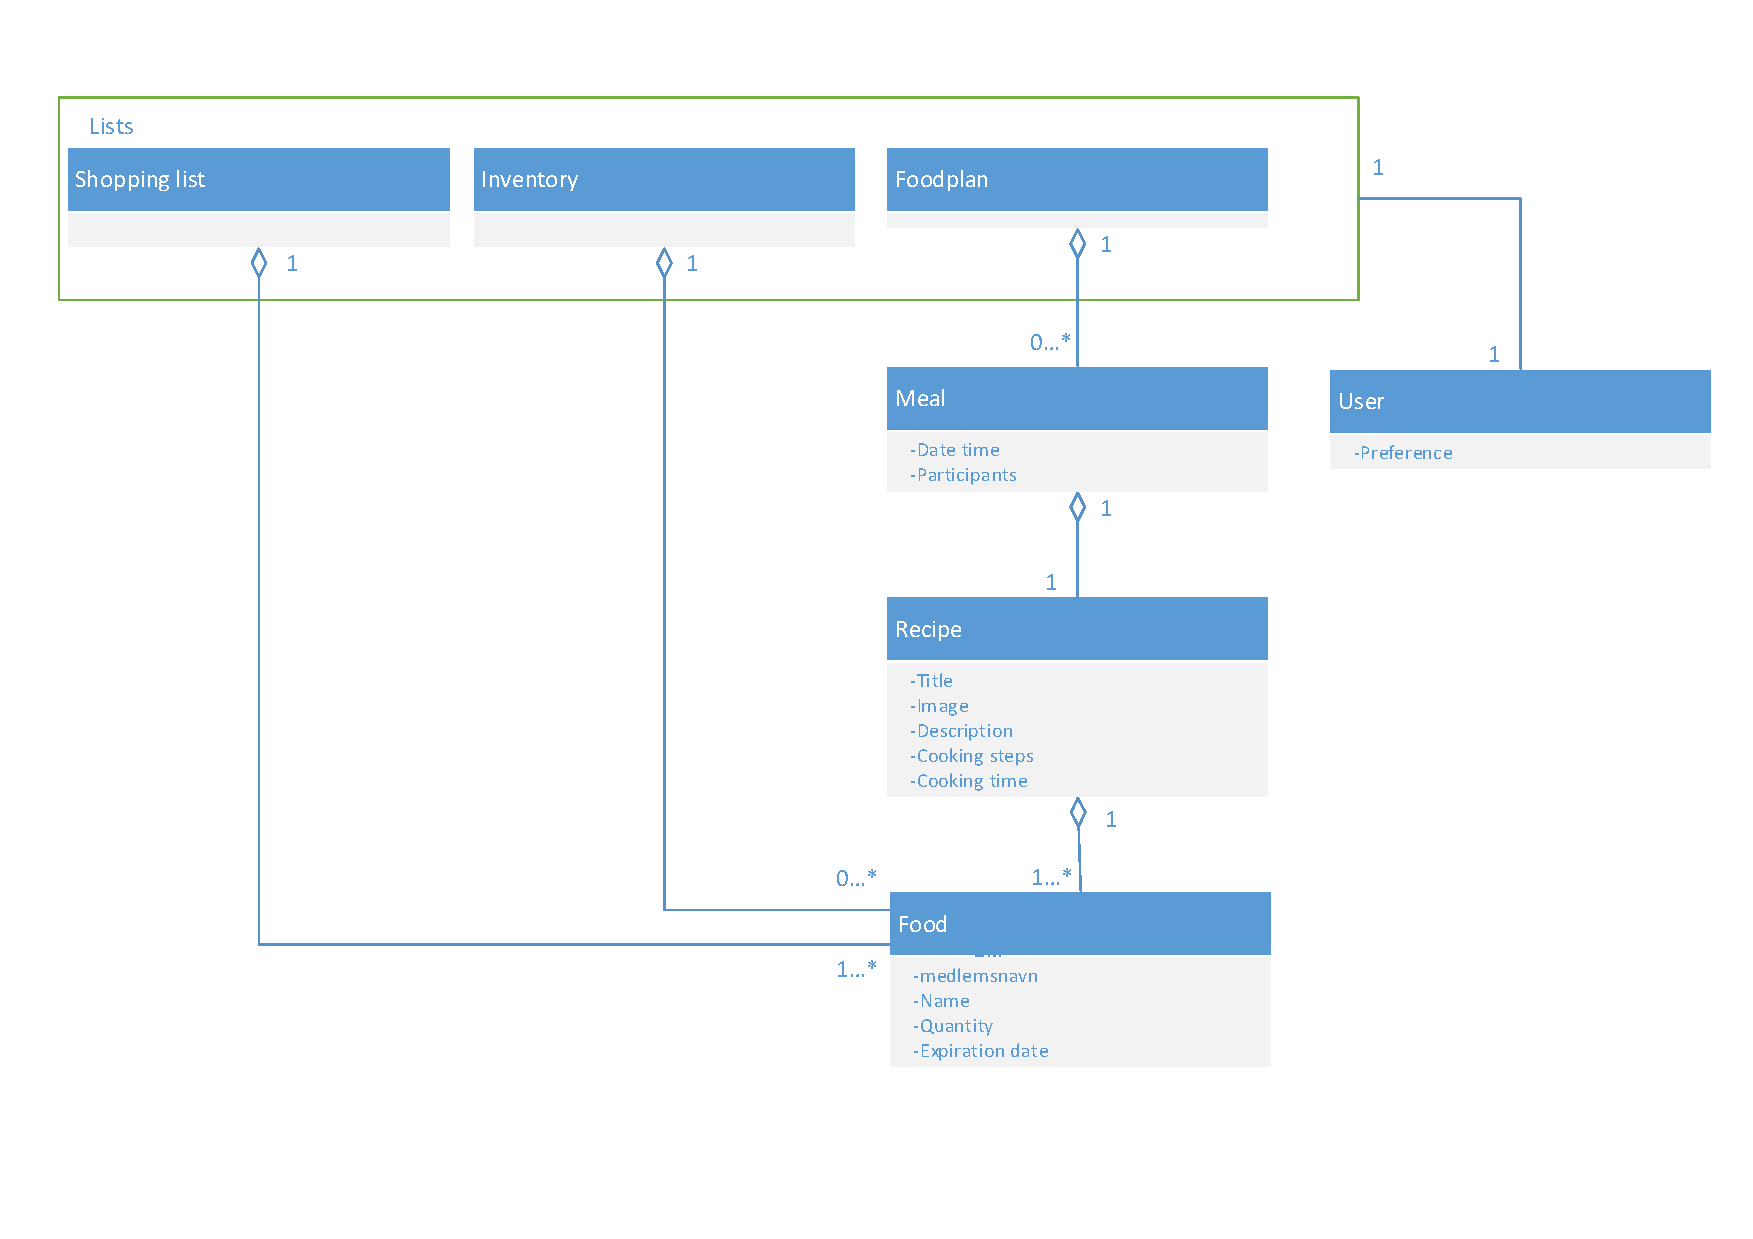
\includegraphics[clip=true, width=1\textwidth, trim=1cm 3cm 4cm 0]{Development/Klasseting}
	\caption{Relation between classes.}
	\label{fig:classDiagram} \fxnote{Indeholder ikke User og shopping klassen!}
\end{figure}

\section{Events} \label{EventsSection}
In this section a list of events will be presented. The events described are those which have been chosen through an event candidate analysis. The events and what trigger them are listed below.

\subsection{Event Definitions}

\subsubsection{Consumption}
\begin{itemize}
\item \textbf{Product bought:} A shopping list have been completed. The items bought will be added to an inventory.
\item \textbf{Product removed:} A meal have been prepared and the product should be removed from the inventory, or have an subtraction from its original volume/quantity.
\item \textbf{Product expired:} When a product reaches its expiration date, it should be removed from the inventory and thrown out.
\end{itemize}

\subsubsection{Planning}
\begin{itemize}
    \item \textbf{Recipe scheduled:} When a recipe is scheduled for a date in the meal plan.
    \item \textbf{Recipe removed:} When the user removes a recipe which was scheduled for a date in the meal plan.
    \item \textbf{Shopping list item added:} When a recipe have been scheduled in the meal plan, missing ingredients from the inventory are added to the shopping list.
\end{itemize}

\subsubsection{Preferences/settings}
\begin{itemize}
\item \textbf{Preference changed:} When the user navigates to a settings menu to exclude products from the system, due to allergies, diets or preference.
\end{itemize}

\section{Event Table}
\Cref{tab:EventTable} shows an event table that have been constructed in order to get an overview of the relations between classes and events. The event table allows for a better judgement of which classes are relevant in the program. A plus (+) in the table indicates, that an event can occur zero or one time, whereas a star (*) indicates that an event can occur zero or more times.

\begin{table}[H]\centering
    \begin{tabular}{|r|c|c|c|c|}
        \hline
        ~                                      & Product & Recipe & User & Meal\\ \hline
        \textbf{Consumption}                   & ~       & ~      & ~    & ~   \\ 
		    Product added                          & +       & ~      & ~    & ~   \\ 
        Product removed                        & +       & ~      & ~    & ~   \\ 
        Product expired                        & *       & ~      & ~    & ~   \\ 
        Product unexpired                      & *       & ~      & ~    & ~   \\ 
        Product quantity changed               & *       & ~      & ~    & ~   \\ 
        Product expiration changed             & *       & ~      & ~    & ~   \\ 
        \textbf{Planning}                      & ~       & ~      & ~    & ~   \\ 
        Shopping list item added               & +       & ~      & ~    & ~   \\ 
        Meal added                             & ~       & +      & ~    & +   \\ 
        Meal removed                           & ~       & +      & ~    & +   \\ 
        Meal rescheduled                       & ~       & +      & ~    & +   \\ 
        Meal participants changed              & ~       & ~      & ~    & *   \\ 
        Meal Date changed                      & ~       & ~      & ~    & *   \\ 
        \textbf{Other}                         & ~       & ~      & ~    & ~   \\ 
        Preference changed                     & ~       & ~      & *    & ~   \\ 
		    Recipe found                           & ~       & *      & ~    & ~   \\ 
		\hline    
    \end{tabular}
    \caption{An event table for the program} 
    \label{tab:EventTable}
\end{table}